\documentclass[12pt]{article}
\renewcommand{\familydefault}{\sfdefault} % Sans-serif font

\usepackage[a4paper, margin=1in]{geometry}
\usepackage[colorlinks=true, linkcolor=blue, urlcolor=blue]{hyperref}
\usepackage{listings}
\usepackage{xcolor}
\usepackage{tcolorbox}
\usepackage{longtable}
\usepackage{graphicx}
\usepackage{pdflscape}

% Setup for code
\lstset{
  basicstyle=\ttfamily\small,
  backgroundcolor=\color{gray!10},
  frame=single,
  breaklines=true
}

% Custom note box
\newtcolorbox{noteBox}{
  colback=yellow!10,
colframe=orange!60!black,
  title=Note,
  fonttitle=\bfseries
}

\begin{document}

% --- Title Page ---
\begin{titlepage}
  \centering
  \vspace*{\fill}

  {\LARGE\bfseries Software Requirements Specification (SRS)\par}
  \vspace{1cm}

  {\Large Project Team\par}
  \vspace{0.5cm}

  {\large \today\par}

  \vspace*{\fill}
\end{titlepage}

% --- TOC, LOF, LOT ---
\tableofcontents
\listoffigures
\listoftables
\newpage

% --- Main Content ---
\section{Use Case Specifications}
\label{sec:usecases}

This section describes the primary use cases for the system.

\subsection{Use Case: User Login}
\label{sec:login}

\textbf{Brief Description:} Allows users to log into the system using their credentials.

\subsubsection*{Actors}
- Registered User

\subsubsection*{Preconditions}
- The user has already registered.

\subsubsection*{Basic Flow}
\begin{enumerate}
    \item User navigates to the login page.
    \item User enters email and password.
    \item System validates credentials.
    \item User is redirected to the dashboard.
\end{enumerate}

\subsubsection*{Alternate Flow}
If the credentials are invalid:
\begin{itemize}
    \item System displays an error message.
    \item User is asked to retry or reset password.
\end{itemize}

\subsubsection*{Postconditions}
- The user is authenticated and logged in.

% Hyperlink to another section
For more use cases, see Section~\ref{sec:usecases}.

% External hyperlink
For design references, visit \href{https://developer.mozilla.org/en-US/docs/Web/HTTP/Authentication}{MDN Web Docs on Authentication}.

% Add a note
\begin{noteBox}
Use HTTPS to secure login credentials during transmission.
\end{noteBox}

\begin{noteBox}
Test
\end{noteBox}

% Add a code snippet
\subsection*{Sample Login Validation Code (Python)}

\begin{lstlisting}[language=Python, caption=Simple login validation]
def login(email, password):
    user = db.find_user(email)
    if user and user.check_password(password):
        return True
    return False
\end{lstlisting}

% Landscape figure section
\subsection*{Login Flow Diagram}
\clearpage
\begin{landscape}
\begin{figure}[ht]
  \centering
  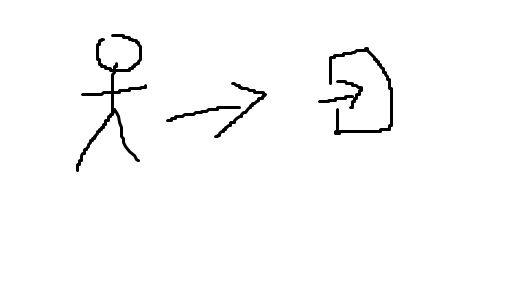
\includegraphics[width=\linewidth]{login_flow.png}
  \caption{Login flow for registered users}
  \label{fig:loginflow}
\end{figure}
\end{landscape}
\clearpage

% Add a table
\subsection*{Use Case Attributes}

\begin{longtable}{|p{4cm}|p{10cm}|}
\caption{User Login Use Case Attributes} \label{tab:login-attributes} \\
\hline
\textbf{Attribute} & \textbf{Description} \\
\hline
Use Case ID & UC-01 \\
\hline
Use Case Name & User Login \\
\hline
Primary Actor & Registered User \\
\hline
Goal in Context & Authenticate user to access secure dashboard \\
\hline
Stakeholders and Interests & Users want secure access; system must ensure data protection \\
\hline
\end{longtable}

\end{document}
